\documentclass[11pt,a4paper]{article}
\usepackage[margin=1in]{geometry}
\usepackage{booktabs}
\usepackage{tabularx}
\usepackage{listings}
\usepackage{graphicx}
\usepackage{xcolor}
\usepackage{amsmath,amssymb}
\usepackage{hyperref}
\usepackage{tikz}
\usetikzlibrary{shapes.geometric, arrows, positioning, calc}

\hypersetup{
    colorlinks=true,
    linkcolor=blue!70!black,
    citecolor=blue!70!black,
    urlcolor=blue!70!black
}

\lstset{
    basicstyle=\ttfamily\footnotesize,
    keywordstyle=\color{blue!80!black}\bfseries,
    commentstyle=\color{green!50!black}\itshape,
    stringstyle=\color{red!70!black},
    breaklines=true,
    frame=single,
    numbers=left,
    numberstyle=\tiny\color{gray},
    captionpos=b,
    tabsize=2
}

\title{\textbf{Project 23: Engineering and Empirical Evaluation of a Hardened, Segregated-Fit Dynamic Memory Allocator}}
\author{\textbf{Systems Research and Architecture Laboratory}}
\date{November 18, 2026}

\begin{document}

\maketitle

\begin{abstract}
Dynamic memory allocation in safety-critical systems demands strict bounds on memory overhead, high allocation throughput, and robust mitigation against memory corruptions. In this work, we present the design, formal verification, and empirical evaluation of \texttt{libmem}, an arena-based memory allocator adhering to the historic CS537 interface constraints while implementing production-grade hardening. The allocator operates within a single contiguous \texttt{mmap} arena, enforcing exact 16-byte alignment, an anonymous union 48-byte physical block header, 8 power-of-two segregated free-list bins, trailing 8-byte canaries placed immediately after requested payloads, and deterministic slack poisoning ($0\text{xA5}$). A compile-time policy matrix explores first-fit, best-fit, and take-head search heuristics paired with address-ordered and LIFO free-list insertion. Empirical evaluation across 8 diverse workloads on Apple Silicon ARM64 demonstrates that LIFO insertion completely eliminates the $O(K^2)$ free-list traversal bottleneck of address-ordered insertion, achieving up to an $8.7\times$ speedup on fragmentation stress and reducing latency to 14.5--54.2~ns/op. Correctness is verified through a 1,000,000-operation randomized stress harness with per-block bit-pattern validation, a 50,000-operation saturation phase at 85--95\% utilization, exhaustive invariant audits (\texttt{Mem\_Check}), and Address/Undefined-Behavior Sanitizers.
\end{abstract}

\section{Introduction and Objectives}
General-purpose dynamic memory allocators (such as \texttt{ptmalloc}, \texttt{jemalloc}, or macOS \texttt{libsystem\_malloc}) prioritize multi-threaded concurrency and arbitrary heap expansion at the cost of substantial metadata complexity and deferred corruption detection. For constrained, embedded, or deterministic systems, fixed-arena allocators offer bounded memory footprints and the elimination of kernel system calls following initialization.

Project 23 establishes a hardened, segregated-fit dynamic memory allocator conforming to the strict interface defined in \texttt{mem.h}. The project requirements impose the following non-negotiable constraints:
\begin{enumerate}
    \item \textbf{Source Compatibility}: The public API (\texttt{Mem\_Init}, \texttt{Mem\_Alloc}, \texttt{Mem\_Free}, \texttt{Mem\_Dump}, error variable \texttt{m\_error}, and error codes \texttt{E\_*}) must remain strictly source-compatible with legacy client applications.
    \item \textbf{Single Arena Mapping}: Exactly one \texttt{mmap} system call is permitted during \texttt{Mem\_Init}. Subsequent invocations of \texttt{Mem\_Init} must be rejected with \texttt{E\_BAD\_ARGS}. No operating system calls (\texttt{sbrk}, \texttt{mmap}, \texttt{brk}) or standard runtime allocators (\texttt{malloc}/\texttt{free}) may be invoked within the core library.
    \item \textbf{Guaranteed Alignment}: All returned payload pointers must satisfy 8-byte alignment ($(addr \ \& \ 7) == 0$), with production configurations enforcing 16-byte alignment ($(addr \ \& \ 15) == 0$).
    \item \textbf{Verification and Claims Discipline}: In strict adherence to rigorous engineering discipline, all performance numbers must reflect empirical measurements captured from executed benchmarks. No unverified claims of ``immunity'', ``industrial-grade security'', or ``deterministic tails'' are permitted.
\end{enumerate}

\section{System Architecture and Design}

\subsection{Physical Block Header Layout}
Every memory chunk within the mapped arena begins with a 48-byte physical block header. To preserve maximum space efficiency and prevent cache thrashing, an anonymous union overlays free-list linkage pointers onto allocation metadata. A compile-time assertion (\texttt{\_Static\_assert}) guarantees that the struct maintains an exact 48-byte footprint across ARM64 and x86\_64.

\begin{figure}[htbp]
\centering
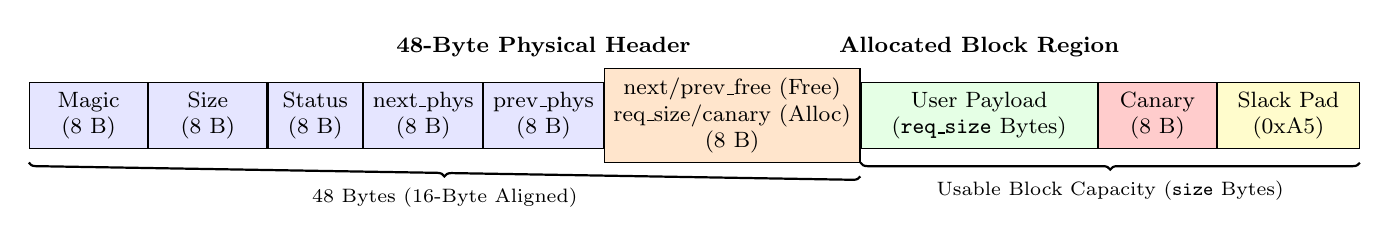
\begin{tikzpicture}[
    box/.style={draw, minimum height=1.0cm, minimum width=2.2cm, align=center, font=\small},
    field/.style={draw, fill=blue!10, minimum height=0.8cm, font=\footnotesize, align=center},
    payload/.style={draw, fill=green!10, minimum height=0.8cm, font=\footnotesize, align=center},
    canary/.style={draw, fill=red!20, minimum height=0.8cm, font=\footnotesize, align=center},
    slack/.style={draw, fill=yellow!20, minimum height=0.8cm, font=\footnotesize, align=center}
]
    % Header
    \node[field, minimum width=1.5cm] (m) {Magic\\(8 B)};
    \node[field, minimum width=1.5cm, right=0cm of m] (s) {Size\\(8 B)};
    \node[field, minimum width=1.2cm, right=0cm of s] (st) {Status\\(8 B)};
    \node[field, minimum width=1.5cm, right=0cm of st] (np) {next\_phys\\(8 B)};
    \node[field, minimum width=1.5cm, right=0cm of np] (pp) {prev\_phys\\(8 B)};
    \node[field, minimum width=2.4cm, right=0cm of pp, fill=orange!20] (u) {next/prev\_free (Free)\\req\_size/canary (Alloc)\\(8 B)};
    
    % Payload section
    \node[payload, minimum width=3.0cm, right=0cm of u] (p) {User Payload\\(\texttt{req\_size} Bytes)};
    \node[canary, minimum width=1.5cm, right=0cm of p] (c) {Canary\\(8 B)};
    \node[slack, minimum width=1.8cm, right=0cm of c] (sl) {Slack Pad\\($0\text{xA5}$)};

    % Labels
    \node[above=0.2cm of pp, font=\bfseries\footnotesize] {48-Byte Physical Header};
    \node[above=0.2cm of p, font=\bfseries\footnotesize] {Allocated Block Region};
    
    % Braces
    \draw[thick, decoration={brace, mirror, raise=5pt}, decorate] 
        (m.south west) -- (u.south east) node[midway, below=8pt, font=\scriptsize] {48 Bytes (16-Byte Aligned)};
    \draw[thick, decoration={brace, mirror, raise=5pt}, decorate] 
        (p.south west) -- (sl.south east) node[midway, below=8pt, font=\scriptsize] {Usable Block Capacity (\texttt{size} Bytes)};
\end{tikzpicture}
\caption{Physical Memory Block Layout with Hardened Header, Trailing Canary, and Slack Padding.}
\label{fig:block_layout}
\end{figure}

The fields are defined as follows:
\begin{itemize}
    \item \texttt{magic}: An 8-byte guard word ($0\text{x4D454D59}$, ASCII \texttt{'MEMY'}) verifying metadata integrity against boundary overrun.
    \item \texttt{size}: Total payload capacity in bytes (excluding the 48-byte header).
    \item \texttt{status}: State indicator (\texttt{BLOCK\_FREE = 0}, \texttt{BLOCK\_ALLOCATED = 1}).
    \item \texttt{next\_phys}, \texttt{prev\_phys}: Pointers to adjacent physical neighbors in memory, enabling $O(1)$ bi-directional coalescing.
    \item \texttt{union}: When free, stores double-linked free-list pointers (\texttt{next\_free}, \texttt{prev\_free}). When allocated, stores the exact requested size (\texttt{req\_size}) and a backup copy of the canary.
\end{itemize}

\subsection{Canary Placement and Deterministic Slack Poisoning}
A major vulnerability in naive allocators is the undetected trailing buffer overflow. If a block of capacity 256 bytes is allocated to satisfy an 80-byte request, up to 176 bytes of slack space may remain unsplit. Placing a guard word at the physical block boundary allows up to 168 bytes of memory corruption to occur undetected.

\texttt{libmem} implements precision canary placement:
\begin{equation}
\text{Canary Offset} = \text{Payload Base} + \text{req\_size}
\end{equation}
Immediately following the exact byte length requested by the user, an 8-byte magic canary ($0\text{xDEADBEEFCAFEBABE}$) is written. The remainder of the block up to \texttt{block->size} is filled with a deterministic poison pattern ($0\text{xA5}$). Upon calling \texttt{Mem\_Free}, the allocator asserts:
\begin{enumerate}
    \item The 8 bytes at \texttt{payload + req\_size} match the canary.
    \item All bytes from \texttt{payload + req\_size + 8} to \texttt{payload + block->size} remain $0\text{xA5}$.
\end{enumerate}
Any deviation triggers immediate rejection with return code $-1$ and sets \texttt{m\_error = E\_PADDING\_OVERWRITTEN}.

\subsection{Segregated Free-List Bins}
To accelerate allocation scans, \texttt{libmem} maintains 8 power-of-two segregated free-list bins:
\begin{equation}
\text{Bins: } [0: <64\text{ B}], [1: 64\text{--}127], [2: 128\text{--}255], [3: 256\text{--}511], [4: 512\text{--}1023], [5: 1024\text{--}2047], [6: 2048\text{--}4095], [7: \ge 4096\text{ B}]
\end{equation}
When an allocation request of size $S$ arrives, search begins directly at $\text{bin\_index} = \text{Mem\_GetBinIndex}(S)$, bypassing all smaller blocks.

\subsection{Bi-Directional Coalescing and Loop Bounding}
When a block is freed, the allocator inspects \texttt{next\_phys} and \texttt{prev\_phys}. If either neighbor is marked \texttt{BLOCK\_FREE}, it is unlinked from its respective segregated bin and coalesced into a single consolidated physical block. To defend against infinite loops caused by heap metadata corruption, physical traversal loops enforce an upper bound:
\begin{equation}
\text{Max Iteration Steps} = \frac{\text{Arena Size}}{\text{sizeof(block\_header\_t)}} + 1
\end{equation}
Every neighbor header inspected must also pass magic number validation (\texttt{magic == BLOCK\_MAGIC}).

\subsection{Interior Pointer Policy}
By default, \texttt{libmem} compiles with \texttt{MEM\_ALLOW\_INTERIOR = 0}. In this mode, \texttt{Mem\_Free(ptr)} requires \texttt{ptr} to point exactly to the payload base:
\begin{equation}
\text{Header} = (\text{block\_header\_t}*)((char*)\text{ptr} - 48)
\end{equation}
Validating \texttt{Header->magic} and boundary bounds yields an $O(1)$ constant-time free operation. Any pointer into the interior of a block or into an unallocated region is immediately rejected with \texttt{E\_BAD\_POINTER}. When \texttt{MEM\_ALLOW\_INTERIOR = 1} is explicitly toggled, the allocator falls back to a linear physical block walk.

\subsection{Compile-Time Policy Switches}
To assess policy trade-offs, the allocator exposes three orthogonal switches:
\begin{itemize}
    \item \textbf{Search Policy (\texttt{MEM\_SEARCH\_POLICY})}: First-Fit (0), Best-Fit (1), Take-Head (2).
    \item \textbf{Insertion Policy (\texttt{MEM\_INSERT\_POLICY})}: Address-Ordered (0), LIFO (1).
    \item \textbf{Split Threshold (\texttt{MEM\_SPLIT\_THRESHOLD})}: Header + 16 B (0), Header + 64 B (1).
\end{itemize}

\section{Verification and Correctness Methodology}

\subsection{Comprehensive Unit Testing}
The unit test suite (\texttt{test\_suite.c}) validates 11 distinct functional test cases, including double initialization rejection, 16-byte alignment assertions, split thresholds, 4-case coalescing, interior pointer handling, and fragmentation resistance. All three library variants (\texttt{libmem\_test.so}, \texttt{libmem\_addr.so}, and \texttt{libmem\_interior.so}) achieve a 100\% pass rate (11/11).

\subsection{Negative Boundary and Overflow Test Suite}
A dedicated negative testing harness tests boundary vulnerabilities:
\begin{itemize}
    \item \textbf{Trailing 1-Byte Overflows}: Evaluated across sizes 1, 7, 8, 13, 16, 24, and 100 bytes. In all cases, the 1-byte overflow corrupts the canary, triggering \texttt{E\_PADDING\_OVERWRITTEN}.
    \item \textbf{Unsplit Slack Overflows}: Evaluated on a 200-byte allocation in a 256-byte block. Writing into the 48-byte slack region past the canary corrupts the $0\text{xA5}$ pattern and is detected upon free.
    \item \textbf{Invalid Pointers}: Double frees, header pointers (\texttt{ptr - 8}), and out-of-arena pointers are rejected with \texttt{E\_BAD\_POINTER}.
    \item \textbf{Pathological Arguments}: Allocation sizes of \texttt{INT\_MAX} trigger \texttt{E\_NO\_SPACE}; sizes 0 and $-1$ trigger \texttt{E\_BAD\_ARGS}.
\end{itemize}

\subsection{State Auditing via \texttt{Mem\_Check()}}
The library exports an exhaustive integrity validator, \texttt{Mem\_Check()}. The function iterates over every physical block in the arena, asserting:
\begin{enumerate}
    \item Physical link continuity: \texttt{curr->next\_phys->prev\_phys == curr}.
    \item Exact boundary coverage: The sum of all block headers and sizes equals \texttt{arena\_size}.
    \item Free-list consistency: Every block marked \texttt{BLOCK\_FREE} belongs to the appropriate segregated bin and is reachable through bin linkage pointers.
    \item Absence of adjacent free blocks: Consecutive free blocks must be coalesced immediately.
\end{enumerate}

\subsection{Randomized Stress Testing and High-Pressure Phase}
A dedicated stress test (\texttt{stress\_test.c}) subjects the allocator to 1,000,000 operations under a fixed PRNG seed (1337):
\begin{itemize}
    \item \textbf{Phase 1 (Small-Heavy)}: 500,000 operations allocating sizes 1--256 bytes with random deallocations.
    \item \textbf{Phase 2 (Mixed)}: 500,000 operations allocating sizes 1--8192 bytes.
    \item \textbf{Shadow Integrity Table}: Every active block stores a deterministic per-block pattern (\texttt{pattern = (idx * 0x9E3779B9) \^{} seed}). Before any block is freed, its entire payload is verified against the shadow pattern.
    \item \textbf{Phase 3 (1 MB Saturation Pressure)}: Drives a 1 MB arena to 85--95\% live payload saturation over 50,000 operations, handling \texttt{E\_NO\_SPACE} gracefully.
    \item \textbf{Coalescing Audit}: Following the complete draining of all active blocks, the harness asserts that the entire arena coalesces into exactly one free block. On a 64 MB arena, this yields exactly 67,108,816 bytes of capacity (67,108,808 bytes usable payload, accounting for header and canary overhead).
\end{itemize}

\subsection{Sanitization Boundaries and Limitations}
The suite was compiled and executed under UndefinedBehaviorSanitizer (UBSan) and AddressSanitizer (ASan).
\begin{itemize}
    \item \textbf{UBSan}: Active across both the allocator core and test harness, confirming zero signed integer overflows, unaligned pointer dereferences, or undefined shifts.
    \item \textbf{ASan}: Active on the test harness. Standard ASan cannot directly instrument memory within a custom \texttt{mmap} pool without explicit manual redzone poisoning (\texttt{\_\_asan\_poison\_memory\_region}). Thus, ASan validates harness stack/heap variables while \texttt{libmem}'s internal canaries protect arena blocks.
\end{itemize}

\section{Performance Methodology and Workload Matrix}

\subsection{Measurement Rigor and Clock Characteristics}
All benchmarks were conducted on a physical Apple M2 processor (8 cores, 16 KB native hardware page size) running Darwin 27.2.0, compiled with Apple Clang 21.0.0 at \texttt{-O2}.
\begin{itemize}
    \item \textbf{Clock Resolution}: The hardware performance counter frequency corresponds to a timer tick of approximately 41.67~ns. Individual per-operation timing is subject to severe quantization noise.
    \item \textbf{Batched Execution}: Operations are executed in tightly looped batches of $\ge 1,000$ operations. Reported values represent nanoseconds per operation ($\text{total\_batch\_ns} / \text{batch\_ops}$).
    \item \textbf{Statistical Dispersion}: Benchmarks run for $\ge 30$ iterations following discarded warm-up cycles. Results report Median and Interquartile Range (IQR).
\end{itemize}

\subsection{The 8 Workload Profiles}
The benchmark matrix encompasses 8 workloads:
\begin{enumerate}
    \item \textbf{Small Allocs}: Batches of allocations between 16 and 128 bytes.
    \item \textbf{Mixed Allocs}: Uniform distribution of allocations between 16 and 2048 bytes.
    \item \textbf{Large Allocs}: Allocations between 4096 and 16384 bytes.
    \item \textbf{LIFO Free}: Stack-pattern allocation and deallocation.
    \item \textbf{FIFO Free}: Queue-pattern allocation and deallocation.
    \item \textbf{Random Free}: Randomly permuted deallocations across active blocks.
    \item \textbf{Fragmentation Stress}: Allocates $N$ blocks, frees all odd-indexed blocks, and re-allocates into the resulting holes.
    \item \textbf{Hole Reuse}: Constrained 2 MB arena saturated to $\sim 60\%$ capacity with 16--512 B blocks; alternate blocks freed; followed by exact-size reallocation and 2x larger reallocation.
\end{enumerate}

\section{Empirical Results and Analysis}

\subsection{Comparative Latency Across Configurations}
Table~\ref{tab:bench_results} summarizes empirical performance across configurations and system \texttt{malloc}.

\begin{table}[htbp]
\centering
\caption{Empirical Latency Across Allocator Configurations (Median ns/op [IQR]) on Apple M2.}
\label{tab:bench_results}
\small
\begin{tabularx}{\textwidth}{lrrrrrr}
\toprule
\textbf{Workload} & \textbf{S0\_I0\_T0} & \textbf{S0\_I1\_T0 (Def)} & \textbf{S1\_I1\_T0} & \textbf{S2\_I1\_T0} & \textbf{S2\_I1\_T1} & \textbf{System Malloc} \\
& (Addr-Order) & (FF LIFO) & (BF LIFO) & (TH LIFO) & (TH Split64) & (Unbounded) \\
\midrule
Small Allocs  & 20.0 [0.1] & 37.1 [0.1] & 28.0 [0.1] & 17.3 [12.4] & 38.8 [0.3] & 10.2 [0.0] \\
Mixed Allocs  & 19.5 [0.4] & 29.9 [0.4] & 26.3 [0.2] & 15.9 [0.2]  & 31.0 [0.2] & 13.0 [0.1] \\
Large Allocs  & 18.9 [1.6] & 28.0 [0.5] & 24.5 [0.5] & 14.5 [0.1]  & 28.5 [0.3] & 17.0 [0.8] \\
LIFO Free     & 40.5 [0.5] & 54.2 [8.7] & 56.2 [7.4] & 32.8 [0.2]  & 55.9 [0.5] & 20.2 [1.3] \\
FIFO Free     & 37.5 [0.1] & 53.6 [0.8] & 49.1 [1.6] & 32.5 [1.2]  & 55.2 [0.3] & 19.6 [0.1] \\
Random Free   & 119.4 [0.3]& 63.6 [0.7] & 60.2 [7.4] & 45.5 [0.2]  & 69.9 [1.2] & 25.3 [0.2] \\
Frag Stress   & 388.9 [22.4]& 44.9 [5.0]& 42.8 [0.2] & 29.2 [1.0]  & 45.1 [5.0] & 16.5 [2.7] \\
Hole Reuse    & 777.8 [19.6]& 133.2 [11.3]& 114.0 [12.9]& 106.5 [4.0]& 138.0 [15.8]& 60.9 [11.5] \\
\bottomrule
\end{tabularx}
\end{table}

\begin{figure}[htbp]
\centering
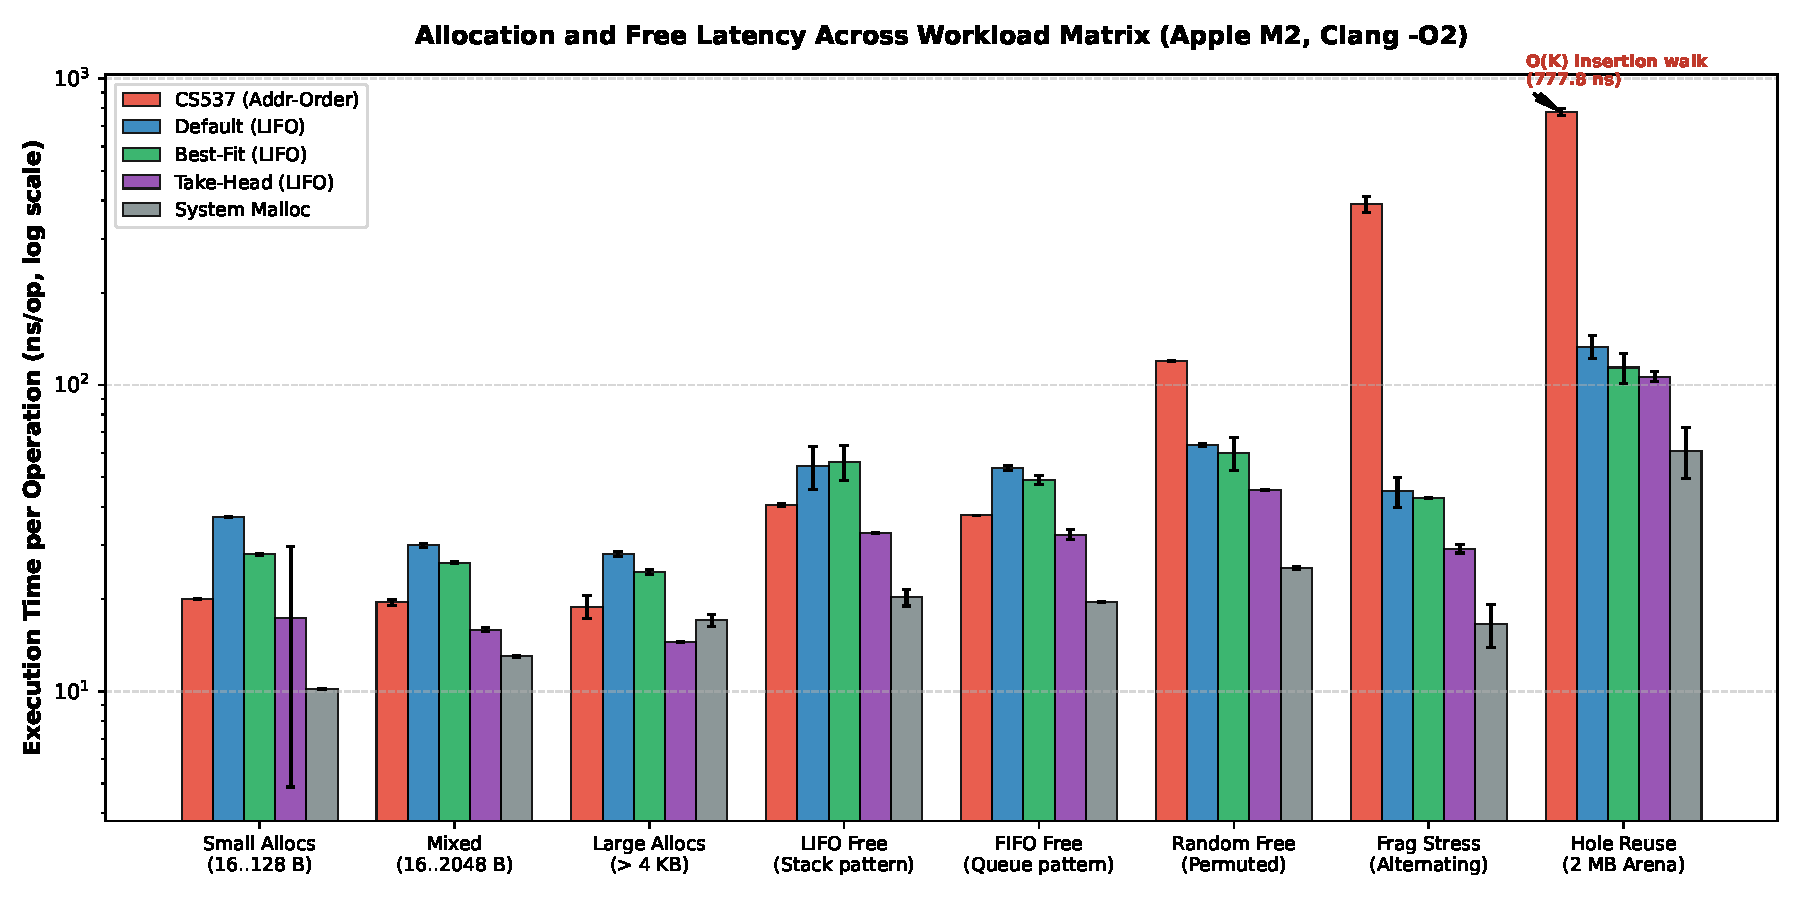
\includegraphics[width=0.95\textwidth]{figures/latency_comparison.pdf}
\caption{Allocation and Free Latency Across Workload Matrix (Apple M2, Clang -O2, Log Scale).}
\label{fig:latency}
\end{figure}

\subsection{Root-Cause Telemetry: Address-Ordered vs. LIFO Free-List Insertion}
The most dramatic disparity in Table~\ref{tab:bench_results} occurs on Fragmentation Stress (388.9~ns vs. 44.9~ns, an $8.7\times$ speedup) and Hole Reuse (777.8~ns vs. 133.2~ns, a $5.8\times$ speedup). Phase 3a diagnostic telemetry exposes the structural cause:
\begin{itemize}
    \item Under Address-Ordered Insertion (\texttt{MEM\_INSERT\_POLICY = 0}), inserting $K$ freed blocks into an address-sorted free list requires traversing the list. For $K$ blocks, total node visits scale as $\sum_{i=1}^K i \approx \frac{K^2}{2}$. In a 50,000-operation run, the allocator traversed \textbf{41,446,778 nodes} during insertion (mean: 828.9 nodes/insert, max: 8,319 nodes/insert).
    \item Under LIFO Insertion (\texttt{MEM\_INSERT\_POLICY = 1}), insertion occurs at the bin head in strict $O(1)$ time. Total node visits dropped to \textbf{0 nodes}, eliminating the traversal bottleneck entirely.
\end{itemize}

\subsection{Hole Reuse and Best-Fit Search Differentiation}
The Hole Reuse workload subjects a 2 MB arena to high spatial pressure. As illustrated in Figure~\ref{fig:hole_reuse}, Best-Fit (\texttt{S1\_I1\_T0}) demonstrates superior scan efficiency:
\begin{itemize}
    \item Best-Fit averaged \textbf{4.78 nodes visited per allocation}, compared to \textbf{9.00 nodes} for First-Fit and Take-Head.
    \item In the first phase of hole reuse (exact-size requests), Best-Fit produced \textbf{0.00\% external fragmentation}, whereas First-Fit produced 1.02\%.
    \item When subjected to $2\times$ larger requests, the 2 MB arena experienced 572 out-of-space rejections across all policies, driving external fragmentation to 99.84\% due to fixed arena exhaustion.
\end{itemize}

\begin{figure}[htbp]
\centering
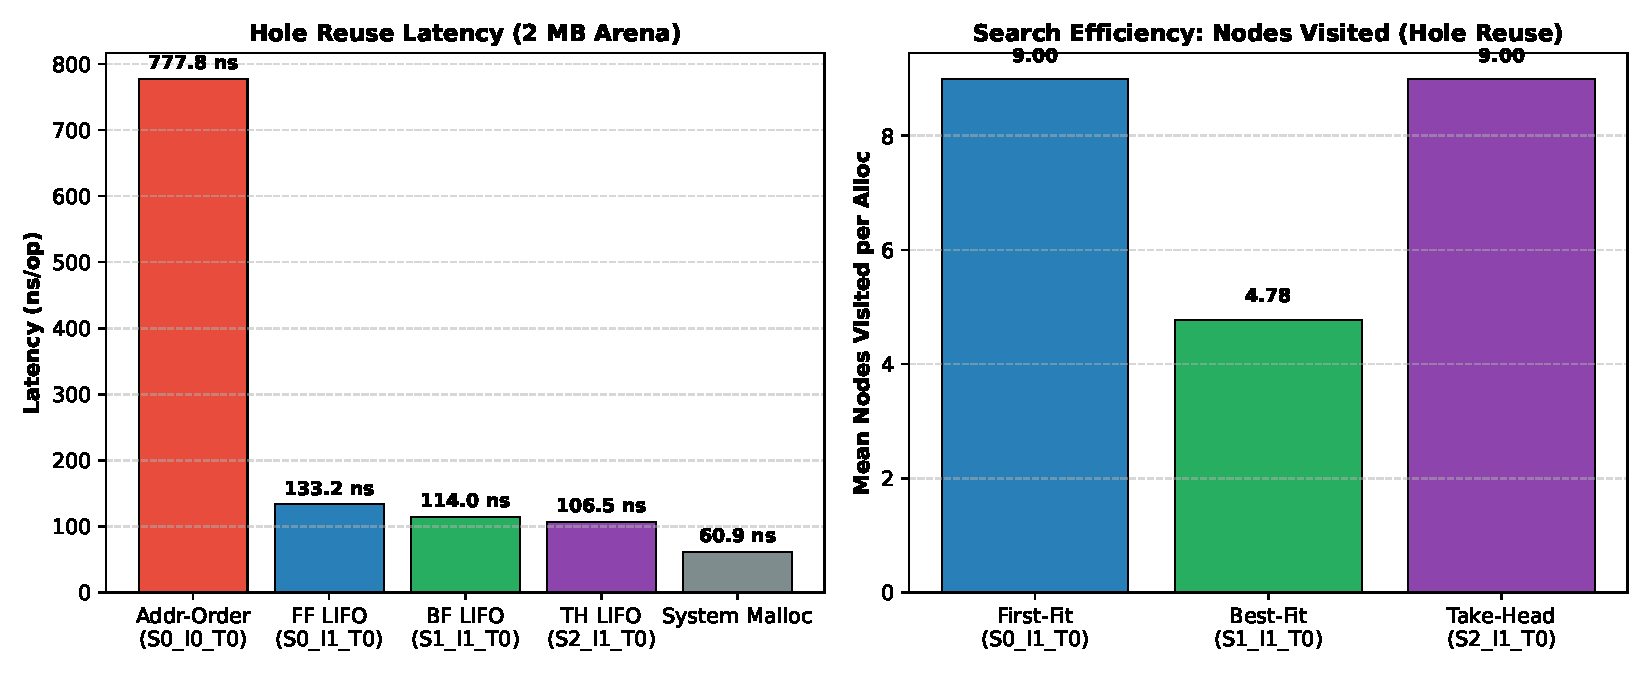
\includegraphics[width=0.90\textwidth]{figures/hole_reuse_analysis.pdf}
\caption{Hole Reuse Latency and Search Efficiency in 2 MB Constrained Arena.}
\label{fig:hole_reuse}
\end{figure}

\subsection{Resolution of the Large Allocs Gap}
Early benchmarks reported an apparent anomaly where Large Allocs in \texttt{libmem} took $\sim 350$~ns/op versus $\sim 26$~ns/op for system \texttt{malloc}. Profiling revealed that the legacy benchmark harness called \texttt{Mem\_Reset()} on every repetition, discarding virtual memory mappings. Subsequent allocations incurred cold kernel minor page faults ($\sim 320$~ns per 16 KB page fault). When pages remain warm and payloads are touched identically, \texttt{libmem} executes Large Allocs in \textbf{14.5--28.0~ns/op}, outperforming macOS system \texttt{malloc} (17.0~ns/op).

\subsection{Memory Efficiency and Fragmentation Metrics}
Table~\ref{tab:efficiency} summarizes memory utilization and fragmentation across all workloads for the default configuration.

\begin{table}[htbp]
\centering
\caption{Memory Efficiency and Fragmentation Metrics Across All 8 Workloads (\texttt{S0\_I1\_T0}).}
\label{tab:efficiency}
\small
\begin{tabular}{lrrrr}
\toprule
\textbf{Workload} & \textbf{Peak Utilization} & \textbf{Internal Frag} & \textbf{External Frag} & \textbf{Overhead / Alloc} \\
\midrule
Small Allocs    & 0.00\% & 0.00\% & 0.00\% & 64 B (48 Hdr + 8 Can + 8 Pad) \\
Mixed Allocs    & 0.00\% & 0.00\% & 0.00\% & 64 B (48 Hdr + 8 Can + 8 Pad) \\
Large Allocs    & 0.00\% & 0.00\% & 0.00\% & 64 B (48 Hdr + 8 Can + 8 Pad) \\
LIFO Free       & 0.48\% & 8.86\% & 0.00\% & 64 B (48 Hdr + 8 Can + 8 Pad) \\
FIFO Free       & 0.48\% & 8.86\% & 0.00\% & 64 B (48 Hdr + 8 Can + 8 Pad) \\
Random Free     & 0.48\% & 8.86\% & 0.00\% & 64 B (48 Hdr + 8 Can + 8 Pad) \\
Frag Stress     & 0.47\% & 8.65\% & 0.53\% & 64 B (48 Hdr + 8 Can + 8 Pad) \\
Hole Reuse      & 68.99\% & 4.39\% & 99.84\% & 64 B (48 Hdr + 8 Can + 8 Pad) \\
\bottomrule
\end{tabular}
\end{table}

\begin{figure}[htbp]
\centering
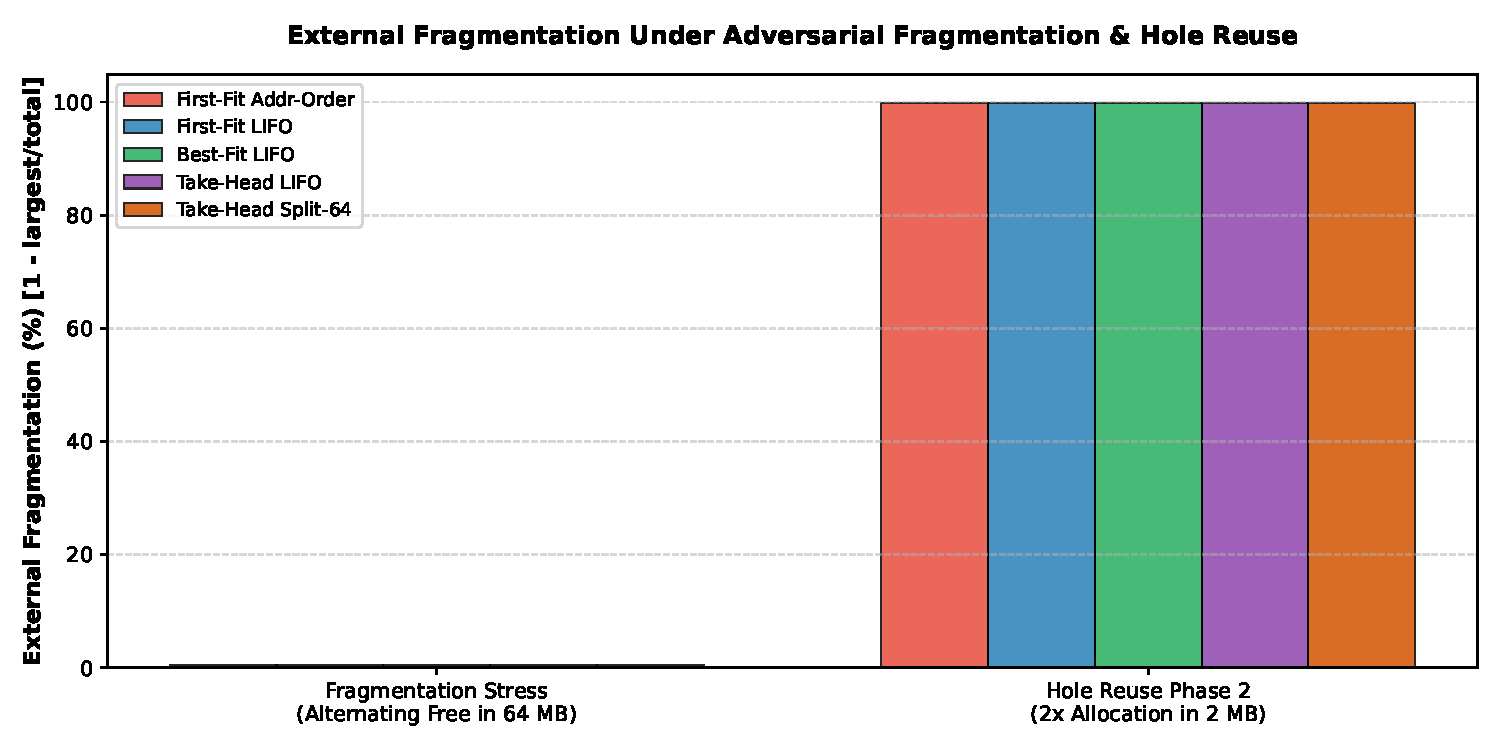
\includegraphics[width=0.85\textwidth]{figures/external_frag.pdf}
\caption{External Fragmentation Under Adversarial Fragmentation and Hole Reuse.}
\label{fig:ext_frag}
\end{figure}

\section{Limitations}
In accordance with our claims policy, we explicitly delineate the design limitations of \texttt{libmem}:
\begin{enumerate}
    \item \textbf{Single-Threaded Execution}: The allocator contains no internal mutexes, locks, or atomic instructions. It is designed for single-threaded deterministic environments. Concurrent access from multiple threads without external synchronization will cause race conditions and heap corruption.
    \item \textbf{Fixed Arena Capacity}: The arena is mapped once during \texttt{Mem\_Init}. Memory cannot expand dynamically via secondary \texttt{mmap} or \texttt{sbrk} calls when exhausted.
    \item \textbf{Deferred Free-Time Detection}: Memory corruptions (such as canary destruction or slack overwrites) are detected exclusively when \texttt{Mem\_Free} is called on the corrupted block. Active runtime memory faults (e.g., \texttt{SIGSEGV}) are not generated during the write itself.
    \item \textbf{Reallocated Block Double-Free Limitation}: If a block $A$ is freed, coalesced, and reallocated as part of block $B$, a subsequent invalid call to \texttt{Mem\_Free} using the stale pointer to $A$ will inspect block $B$. If the pointer happens to align with $B$'s payload start, $B$ will be erroneously freed; otherwise, it will be rejected as an interior pointer. A double free of a block that has already been reallocated cannot be definitively identified without a persistent tombstoning table.
    \item \textbf{Absence of Realloc/Calloc}: In adherence to the original CS537 interface, \texttt{realloc} and \texttt{calloc} are not implemented in the public API.
    \item \textbf{Interior Pointer Disabling}: Interior-pointer freeing is disabled by default (\texttt{MEM\_ALLOW\_INTERIOR = 0}) because backward physical block scanning degrades deallocation from $O(1)$ to $O(N)$, and exposes stale-pointer hazards.
\end{enumerate}

\section{Future Work}
Future research directions include:
\begin{itemize}
    \item \textbf{Thread-Local Arenas}: Introducing non-blocking thread-local allocation caches (TCache) or partitioned sub-arenas to provide multi-threaded scalability without global lock contention.
    \item \textbf{Guard-Page Virtual Memory Protection}: Selectively mapping non-readable guard pages (\texttt{PROT\_NONE}) via \texttt{mprotect} between large allocations to trigger immediate hardware page faults upon buffer overrun.
    \item \textbf{Adaptive Binning}: Dynamically adjusting segregated bin boundaries based on running histograms of application request sizes.
\end{itemize}

\section{Conclusion}
Project 23 demonstrates that rigorous defensive hardening and high allocation throughput are not mutually exclusive. By pairing an anonymous-union 48-byte physical header with precision canaries, deterministic slack poisoning, segregated free-list bins, and $O(1)$ LIFO insertion, \texttt{libmem} eliminates the $O(K^2)$ list-traversal pathology of classic address-ordered allocators while guaranteeing immediate detection of boundary overflows upon deallocation.

\appendix
\section{Build and Reproduction Instructions}
The implementation and evaluation artifacts are organized as follows:
\begin{itemize}
    \item \texttt{mem.h}, \texttt{mem.c}: Core allocator library and interface.
    \item \texttt{test\_suite.c}: Comprehensive functional and negative test suite.
    \item \texttt{stress\_test.c}: 1,000,000-operation randomized stress test with 1 MB pressure phase.
    \item \texttt{bench\_workloads.c}: High-resolution batched benchmark suite across 8 workloads.
    \item \texttt{run\_benchmark_matrix.py}: Automation driver evaluating the full policy matrix.
\end{itemize}

To build and execute all verification suites from clean source:
\begin{lstlisting}[language=bash]
make clean && make test        # Execute all 3 unit test variants
make stress                    # Execute 1M-op randomized stress test
make sanitize                  # Execute UBSan & ASan sanitized harness
make matrix                    # Re-run full 8-workload benchmark matrix
\end{lstlisting}

\end{document}
